\documentclass{beamer}
\usecolortheme{dolphin}
\usepackage{graphics}
\usepackage{graphicx}
\usepackage{listings}
\usepackage{amsmath}
\usepackage{fancyvrb}
\usepackage{color}
\usepackage[ascii]{inputenc}

\lstset{language=Python,
        keywordstyle=\color[rgb]{0,0,1},
        commentstyle=\color[rgb]{0.133,0.545,0.133},
        stringstyle=\color[rgb]{0.627,0.126,0.941},
        columns=fixed,}

\title{Landsat Theater Presentation}
\subtitle{http://github.com/loxodes/fairbanks\_hackathon\_landsat\_viewer}
\author{Jon Klein}
\institute{University of Alaska, Fairbanks}
\date{September 27, 2015}

\begin{document}
    \begin{frame}
        \titlepage
    \end{frame}

    \begin{frame}
        \frametitle{Landsat Theater gathers, process, and displays NASA Landsat imagery}
        \begin{itemize}
            \item Wireless sensor networks operate unattended in hostile environments.
            \item Failures in sensor nodes can result environmental impact, loss of life, or loss of money. 
            \item ``Fault Diagnosis in Wireless Sensor Networks: A Survey'' surveys approaches to detecting faulty sensor nodes.
        \end{itemize}

        \begin{block}{What can we do about faults?}
            \begin{description}
                \item[Fault Detection] is deciding if a specific node is faulty
                \item[Fault Diagnosis] is locating all faulty nodes in a network
                \item[Fault Identification] is estimating the severity and type of a fault
            \end{description}
        \end{block}

    \end{frame}
 
    \begin{frame}
        \frametitle{For software design, I glued together a bunch of open source libraries..}
        \begin{description}
            \item[geopy] for converting cities or addresses to latitude and longitude
            \item[landsat-utils] for downloading and processing landsat data
            \item[Python Image Library] for annotating landsat images with captions
            \item[pyglet] for displaying annotated images
            \item[wx] for the GUI
        \end{description}
    \end{frame}
 
    \begin{frame}
        \frametitle{Landsat Theater could be extended...}
        \begin{itemize}
            \item The tool could clean up after itself, it can easily fill up a hard drive..
            \item The tool lacks error handling and input sanitation.. 
            \item Landsat produces hyperspectral images, some wavelengths could be useful for comparing vegetation
            \item A zoom feature synchronized across all displays would be cool
        \end{itemize}
    \end{frame}

    \begin{frame}
        \frametitle{Landsat is a NASA satellite which captures images of the Earth.}
            \begin{figure}
            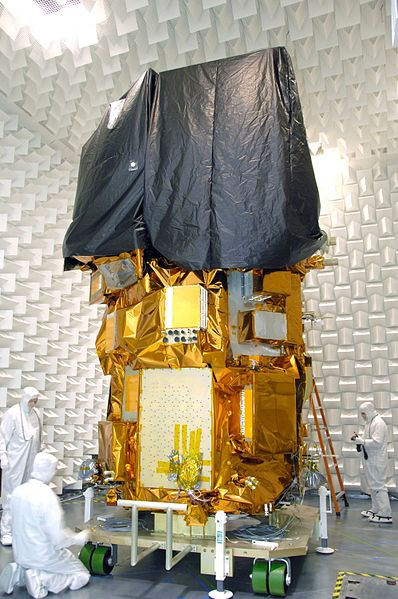
\includegraphics[width=.75\paperheight]{figures/groundlandsat.jpg}
            \caption{Landsat 8 from https://en.wikipedia.org/wiki/Landsat\_8}
            \end{figure}
    \end{frame}

    \begin{frame}
        \frametitle{The imager }
            \begin{figure}
            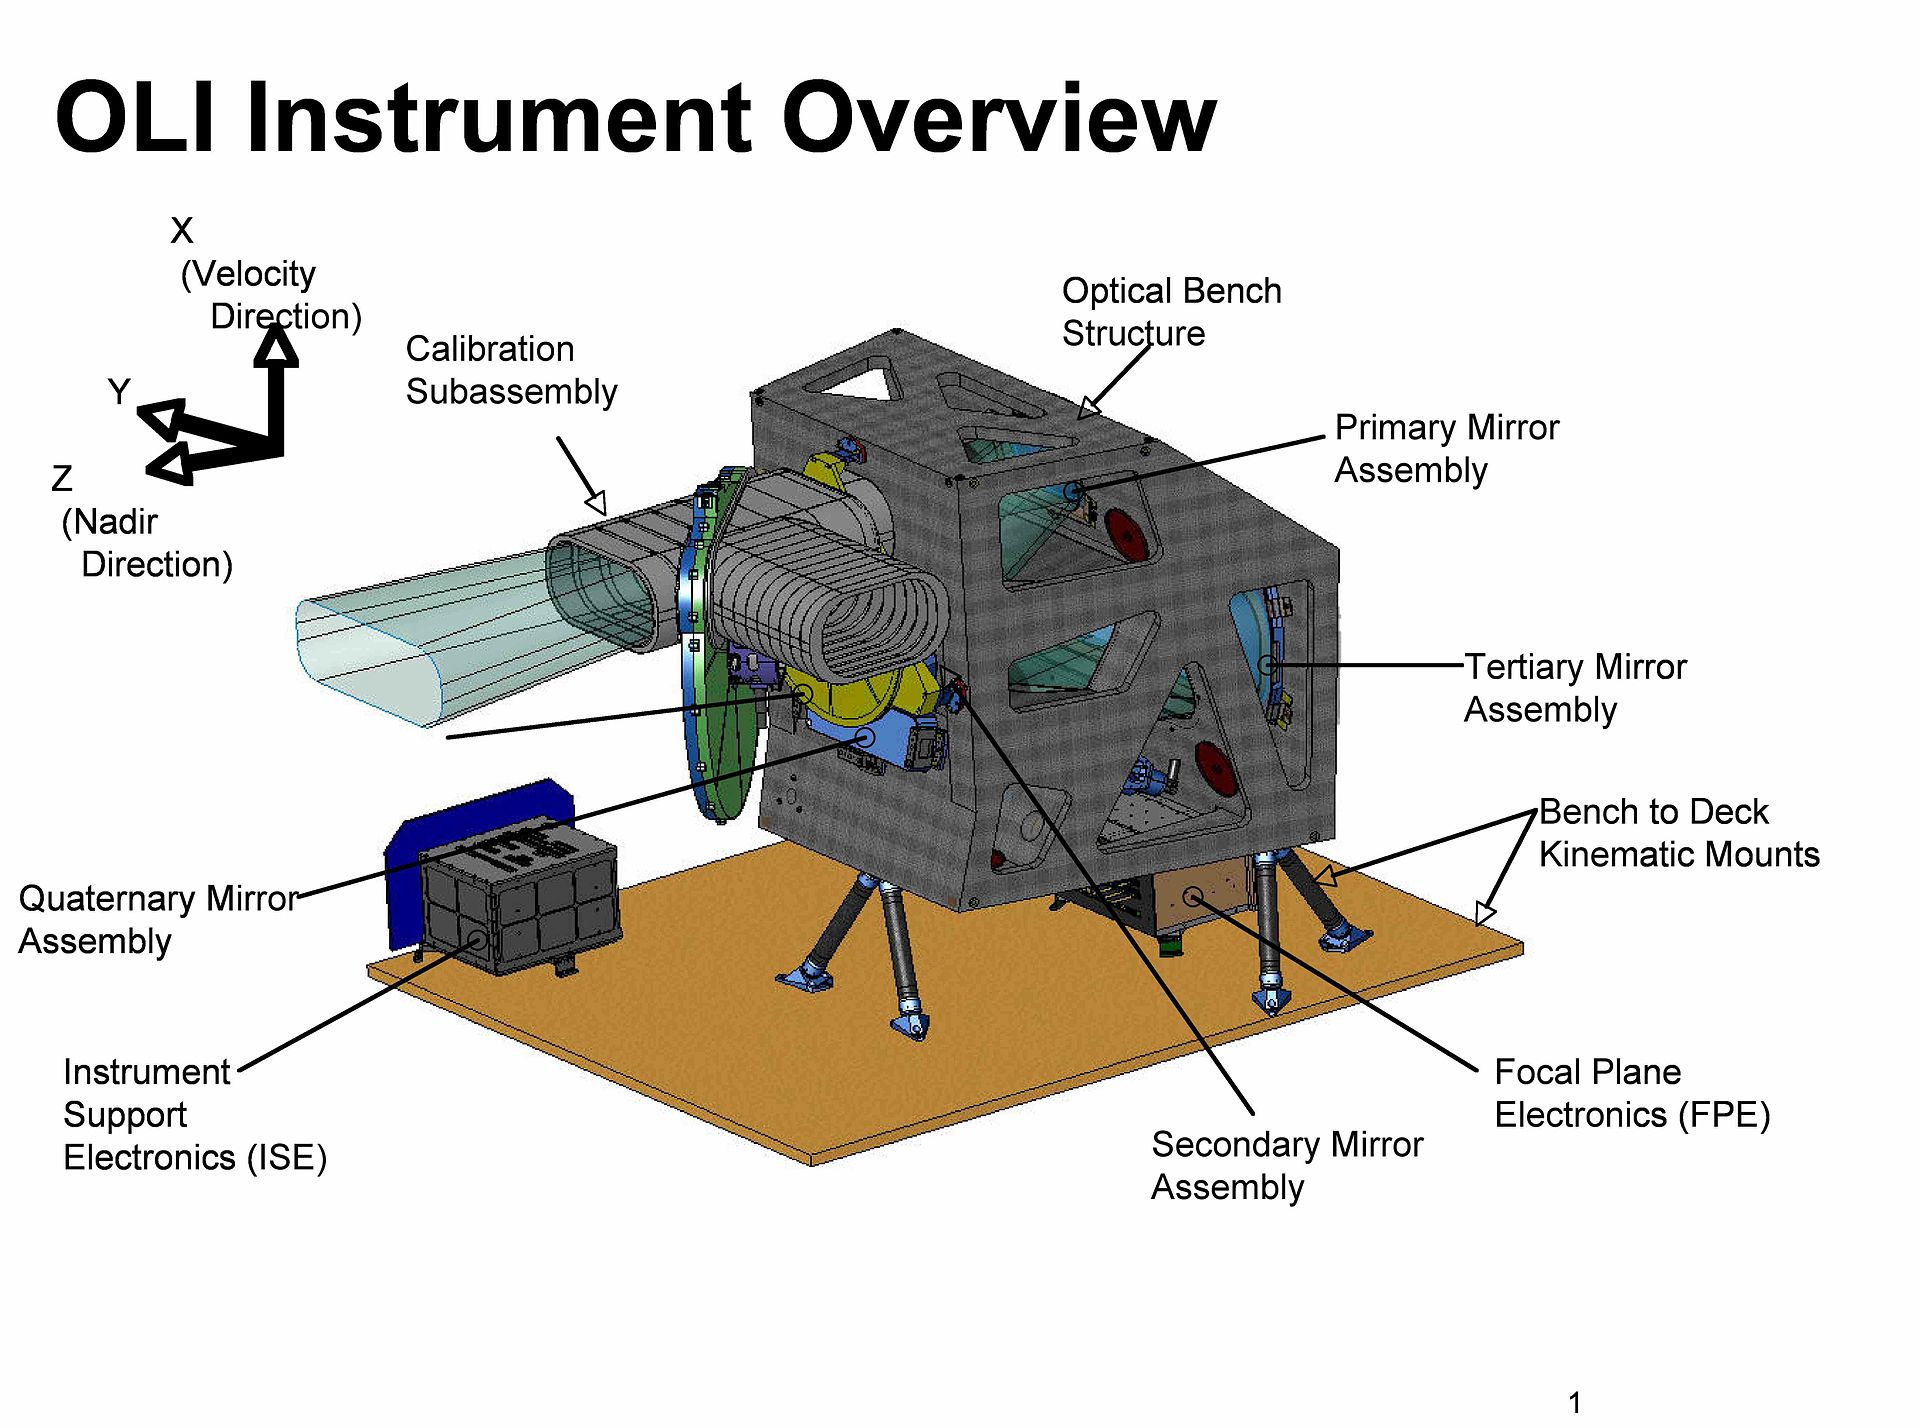
\includegraphics[width=.6\paperheight]{figures/landsatimager.jpg}
            \caption{Watchdog fault diagnosis, node A watches node B relay data to node C [1]}
         \end{figure}


    \end{frame}


    
    \begin{frame}
        \frametitle{Questions?}
        1) Mahapatro, A.; Khilar, P.M., "Fault Diagnosis in Wireless Sensor Networks: A Survey," in Communications Surveys & Tutorials, IEEE , vol.15, no.4, pp.2000-2026, Fourth Quarter 2013
    \end{frame}

\end{document}
